\subsubsection{Quản lý đóng phí}
\begin{figure}[H]
    \centering
    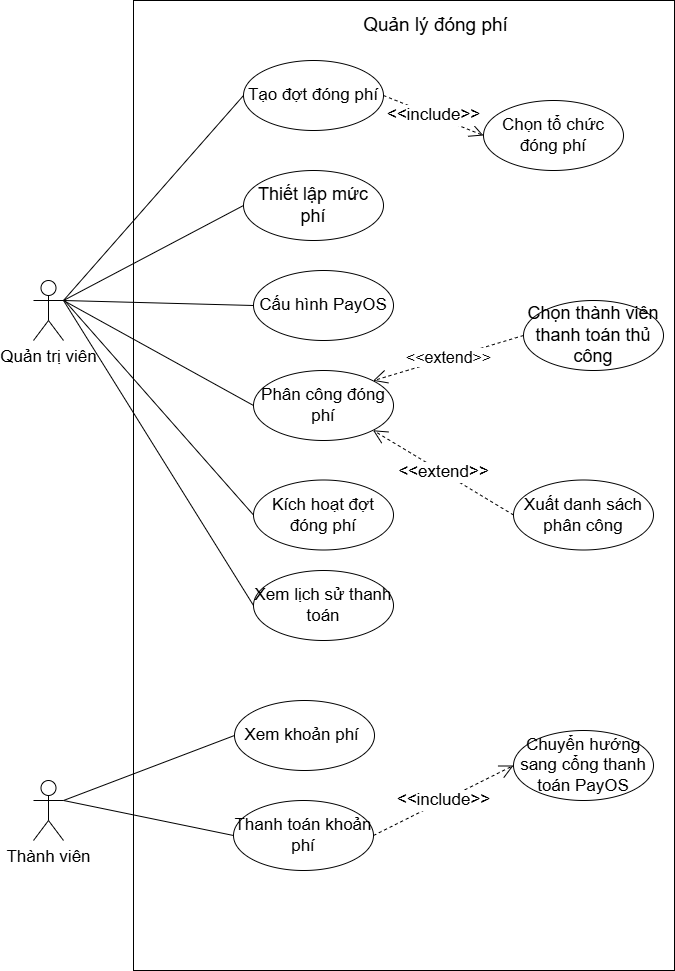
\includegraphics[width=1.0\linewidth]{Images/use-case-diagram/UC04_payment_usecase.drawio.png}
    \vspace{0.3em}
    \caption{UC04 - Quản lý đóng phí}
    \label{fig:uc01-usecase}
\end{figure}
%----------------- Bảng mô tả use case -------------------------------
\renewcommand{\arraystretch}{1.3}
\begin{longtable}{|m{0.25\textwidth}|m{0.75\textwidth}|}
\hline

\textbf{Use Case Name} 
& \textbf{UC04. Quản lý đóng phí} \\ \hline
\endfirsthead

\hline
\textbf{Use Case Name (tiếp)} 
& \textbf{UC04. Quản lý đóng phí} \\ \hline
\endhead

\textbf{Actors} 
& Quản trị viên, Thành viên \\ \hline

\textbf{Description} 
& Quản trị viên tạo một đợt đóng phí mới, thiết lập các thông tin cấu hình cần thiết sau đó kích hoạt đợt đóng phí để thành viên có thể bắt đầu thực hiện thanh toán. 
\\ \hline

\textbf{Trigger} 
& Quản trị viên muốn tạo và khởi động một đợt thu phí mới. 
\\ \hline

\textbf{Pre-Conditions} 
& 
\begin{itemize}
    \item Quản trị viên đã đăng nhập vào hệ thống.
    \item Hệ thống hiện đã có danh sách tổ chức và thành viên để tạo đợt đóng phí và phân công.
\end{itemize}
\\ \hline

\textbf{Post-Conditions} 
& 
\begin{itemize}
    \item Đợt đóng phí mới đã được tạo và lưu lại.
    \item Đợt đóng phí được chuyển từ trạng thái \textit{Nháp} sang \textit{Đang hoạt động}.
    \item Thông tin đợt đóng phí hiển thị trên trang của các thành viên được phân công.
    \item Thành viên thực hiện thanh toán và hệ thống cập nhật trạng thái thanh toán.
\end{itemize}
\\ \hline

\textbf{Normal Flow} 
& 
\begin{enumerate}
    \item Quản trị viên chọn chức năng tạo đợt đóng phí mới.
    \item Hệ thống hiển thị giao diện tạo đợt đóng phí, trạng thái mặc định là \textit{Nháp}.
    \item Quản trị viên điền các thông tin của đợt đóng phí và bấm nút \textit{Lưu}.
    \item Hệ thống lưu đợt đóng phí với trạng thái bản nháp và chuyển hướng đến trang chi tiết đợt đóng phí vừa tạo.
    \item Quản trị viên truy cập tab \textit{Mức phí}, nhập ít nhất một mức phí và lưu lại.
    \item Quản trị viên truy cập tab \textit{Phân công thành viên}, chọn và phân công ít nhất một thành viên và lưu lại.
    \item Quản trị viên truy cập tab \textit{Cấu hình PayOS}, thiết lập API key của cổng thanh toán PayOS và lưu lại.
    \item Quản trị viên nhấn nút \textit{Kích hoạt đợt đóng phí}.
    \item Hệ thống chuyển trạng thái đợt đóng phí từ \textit{Nháp} sang \textit{Đang hoạt động} và hiển thị thông tin đóng phí trên trang \textit{Đóng phí của tôi} của thành viên.
    \item Thành viên truy cập trang \textit{Đóng phí của tôi} và xem các khoản phí cần thanh toán.
    \item Thành viên bấm nút \textit{Thanh toán ngay}, hệ thống chuyển sang cổng thanh toán trực tuyến.
    \item Sau khi thanh toán, hệ thống chuyển về trang kết quả thanh toán và cập nhật trạng thái thanh toán.
\end{enumerate}
\\ \hline

\textbf{Alternative Flow} 
& Ở bước 11:
\begin{itemize}
    \item \textbf{11a.} Thành viên không thanh toán trực tuyến mà đến văn phòng Đoàn để đóng tiền mặt.
    \item \textbf{11b.} Tại trang phân công đóng phí, quản trị viên bấm chọn \textit{Đóng phí thủ công} tại tên thành viên trong danh sách.
    \item \textbf{11c.} Hệ thống cập nhật trạng thái thanh toán của thành viên là \textit{Đã đóng phí (thủ công)}.
\end{itemize}
\\ \hline

\textbf{Exception} 
& Ở bước 8:
\begin{itemize}
    \item \textbf{8a.} Nếu đợt đóng phí thiếu một trong hai cấu hình bắt buộc (\textit{Mức phí} hoặc \textit{Phân công}), nút \textit{Kích hoạt} sẽ không hiển thị.
    \item \textbf{8b.} Hệ thống hiển thị thông báo yêu cầu cấu hình đầy đủ mức phí và phân công thành viên trước khi kích hoạt.
\end{itemize}
\\ \hline
\caption{Bảng mô tả Use Case UC04 - Quản lý đóng phí}
\end{longtable}

